% !TEX program = lualatex
% !TEX spellcheck = it_IT
% !TEX root = ../tlinstall.tex

\section{Manutenzione}

\begin{figure}
\centering
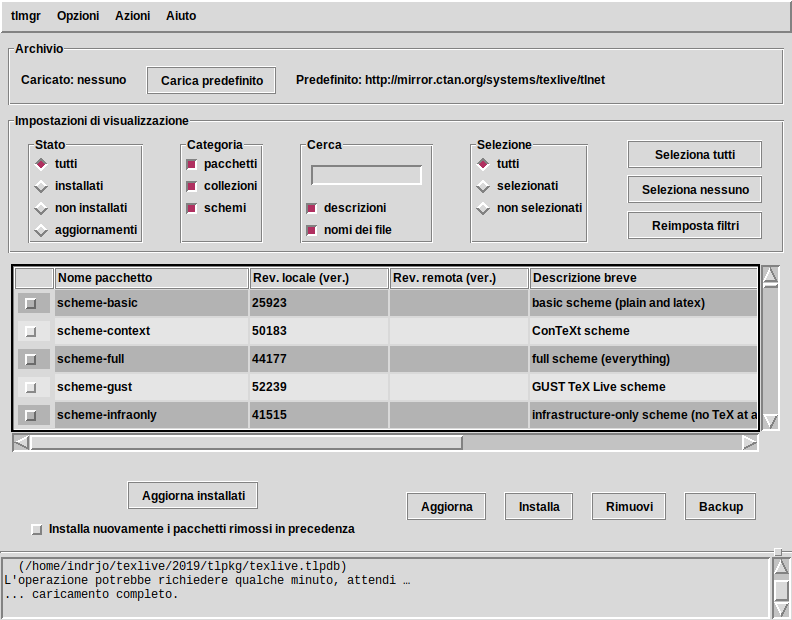
\includegraphics[width=.7\textwidth]{tlmgr}
\caption{\tt tlmgr gui}
\label{fig:gui}
\end{figure}

Diamo qualche breve suggerimento per la manutenzione di \texlive{}. Il programma che ci aiuta in ciò si chiama {\sf tlmgr}. Per averlo pronto all'uso, in fondo al file \lstinline£~/.bash_aliases£ aggiungiamo
\begin{lstlisting}
alias tlmgr='sudo env PATH=$PATH tlmgr'
\end{lstlisting}
da usare nel terminale come
\begin{lstlisting}
tlmgr ?!qualcosa!?
\end{lstlisting}
L'azione che vogliamo insegnare in questa sede è quella dell'aggiornamento dei pacchetti. Per aggiornare se stesso (perché qualche volta ne ha bisogno) dare
\begin{lstlisting}
tlmgr update --self
\end{lstlisting}
Per sapere quali pacchetti hanno bisogno di essere aggiornati (nessuno ci obbliga ad aggiornarli, ma è sempre meglio farlo) fare eseguire questo comando
\begin{lstlisting}
tlmgr update --list
\end{lstlisting}
e per aggiornare tutti quelli che sono aggiornabili
\begin{lstlisting}
tlmgr update --all
\end{lstlisting}
Il consiglio è, finita la procedura di installazione, di aggiornare {\sf tlmgr} stesso e di aggiornare, se possibile, tutti i pacchetti aggiornabili: questo perché nella \lstinline£texlive.iso£ tutto è congelato allo stesso e identico stato del rilascio, col rischio di trovarsi materiale non aggiornato. Se si vuole aggiornare un singolo pacchetto, si può usare
\begin{lstlisting}
tlmgr update ?!nome pacchetto!?
\end{lstlisting}

%\begin{nota}
Se il terminale fa ancora paura, si può optare per questa alternativa
\begin{lstlisting}
tlmgr gui
\end{lstlisting}
che apre la finestra in figura~\ref{fig:gui}. Da lì si possono fare tutte le azioni appena viste e anche altre. Serve che ci sia il modulo {\sf Tk}, però: per installarlo da terminale
\begin{lstlisting}
cpan -f Tk
\end{lstlisting}
%\end{nota}
